\section{Experiments}
\label{sec:exp}

In this section, we conducted experiments to evaluate the effectiveness of applying causal relationships to two tasks: Early Detection of Depression and Diagnosis Point Detection, comparing the results with baseline models.

\subsection{Early Risk Detection of Depression (ERD)}
\paragraph{Dataset} We utilize an ERD dataset proposed by~\citet{chen-etal-2023-detection}. Users and posts were extracted from a publicly available Reddit corpus. The dataset select depression users by detection patterns which consist of two components: one that matches a self-reported diagnosis (e.g., “diagnosed with”), and another that maps relevant keywords to the depression (e.g., major depressive disorder). Control users (i.e., healthy persons) are randomly sampled from those who never posted or commented in mental health related subreddits. The dataset consists of 3,105 users with depression and 17,209 control users.
\paragraph{Baseline} We employ \textbf{PsySym}~\cite{Zhang2022SymptomIF} as baseline, which utilizes CNN of various kernel sizes as backbone, and the inputs are extracted psychiatric symptom features the same as this work. This symptom-based baseline can outperform lots of pure-text methods including BERT-based ones~\cite{nguyen-etal-2022-improving}.
\paragraph{Evaluation Metric} We use the official metrics $ERDE_5$ and $ERDE_{50}$ for Early Detection task proposed by \citet{losada2016test}. The lower $ERDE_5$ and $ERDE_{50}$, the better model performs early detection, and $ERDE_5$ has a higher penalty than $ERDE_{50}$ for late detection. Detailed introduction of these metrics can be found in Appendix \ref{sec:appendixC}. 

\paragraph{Experiment Results} 
We conduct three runs for each method using different seed values, and the results of ERD task is demonstrated in Table \ref{tab:early_detection}. We implement \textit{+symp} by adjusting users' original symptom sequences based on ``symptom-to-symptom'' causality, and \textit{+symp\&LE} incorporates both types of causal relationships.
Generally, we can see that the early detection result can benefit from our methods that applies causality to fulfill the incomplete symptom sequences. 

For the two model variants, they perform comparably on $ERDE_{50}$, while \textit{+symp\&LE} perform better on the more latency-sensitive metric $ERDE_{5}$.
For different causal window size, shorter ones (e.g., 30, 90) are more effective in this task emphasizing low latency. This may be attributed to the fact that causality inferred from a shorter window size is more immediate, enabling the timely identification of potential indicators for early detection. 
% Moreover, the causal relationships inferred from long causal window (i.e., 180) usually 

% // siyuan: not sure about how to analyse causal relationship of LE...
% What's more, 

% % \MY{You have to say more for results. i.e. ERDE5 and 50 have different preferences for symptom causal windows, shorter windows' causality are more helpful for ... By contrast, when combined with LE xxx \KZ{LE stands for Life Event? Define it when first use it.}. Generally with shorter window size, the causal relation is more ... }

\begin{table}[!ht]
    \small
    \centering
    \begin{tabular}{m{1.4cm}|m{1.15cm}|m{1.7cm}|m{1.5cm}}\hline
    Method & CW & $ERDE_5$ & $ERDE_{50}$ \\ 
    \hline
    baseline & - & 13.62$\pm.006$ & 6.72$\pm.105$    \\ \hline
    \multirow{3}*{\textit{+symp}}
    &30 days& 13.49$\pm.013$ & \textbf{6.07}$\pm.092^*$	  \\ 
    &90 days & 13.29$\pm.020^{**}$ & 6.36$\pm.220$   \\
    &180 days & 13.58$\pm.028$ & 7.41$\pm.126$  \\ \hline
    \multirow{3}*{\textit{+symp\&LE}}
    &30 days & 13.42$\pm.014^{*}$ & 6.27$\pm.158$	  \\
    &90 days & \textbf{13.20}$\pm.020^{**}$ & 6.60$\pm.273$    \\
    &180 days & 13.63$\pm.047$ & 6.72$\pm.137$   \\
    \hline
    \end{tabular}
\caption{Results of ERD Task. ``CW'' means ``causal window'', whose definition\textsuperscript{\ref{footnote:causal_window}} can be found in Section \ref{sec:psm}. \textit{symp} is short for ``symptom'', and \textit{LE} is short for ``life event''. The p-values indicating the significance of the differences between the baseline and our method is demonstrated as ($^*$):p<0.1, ($^{**}$):p<0.05}
    \label{tab:early_detection}
\end{table}
% \KZ{Caption? The advantage in ERDE5 is not that obvious. How do we convince people that with symp and LE, it's actually better?}

\paragraph{Case Study}
% \begin{table*}[t]
% \centering
% \scriptsize
% \begin{tabular}{c|p{10cm}|c}
% \hline
% \textbf{ID} & \multicolumn{1}{c}{\textbf{Post}} & \textbf{Life Events} \\
% \hline
% A & Recently, I left my retail job. And I've grappled with depression and anxiety throughout my life. Unfortunately, I can't afford counseling or medication. & \makecell{Health and Well-being,\\ Work and Career Challenges} \\
% \hline
% \end{tabular}
% \caption{We selected a time point on predicted peak and show some representative posts and LEs mentioned \MY{This table is not very informative. You might need to involve more posts of this user to illustrate the peak in a temporal format, like a timeline. If this table is only a complementary to figure6, i suggest you merge it in the figure}}
% \label{case_ERD_table}
% \end{table*}

To assess the effectiveness of incorporating the causal relationships in ERD, we visualize the predicted risk score of one user before and after the inclusion of both two type of causal relationships in Figure \ref{fig:case_ERD}. It clearly demonstrates that after incorporation the causal relations, the predicted risk score surpass the detection threshold (0.5) at an earlier stage compared to the baseline model, which means the model can recognize the depression risk earlier. The reason is that the proposed method can recognize indicative life events before symptom manifestations. For example, before point A, the user posted:
\begin{quote}
\small\texttt{``Recently, I left my retail job.''}
\end{quote}
which matches the ``\textit{Work and Career Challenges}'' life event. The LE-symptom causal relationship will indicate higher risk of depression in the future, facilitating earlier detection. Therefore, even when users do not explicitly express depressive symptoms, our approach, leveraging the association between life events and symptoms, enables us to sensitively capture latent signs of depression. 
\begin{figure}[th]
	\centering
 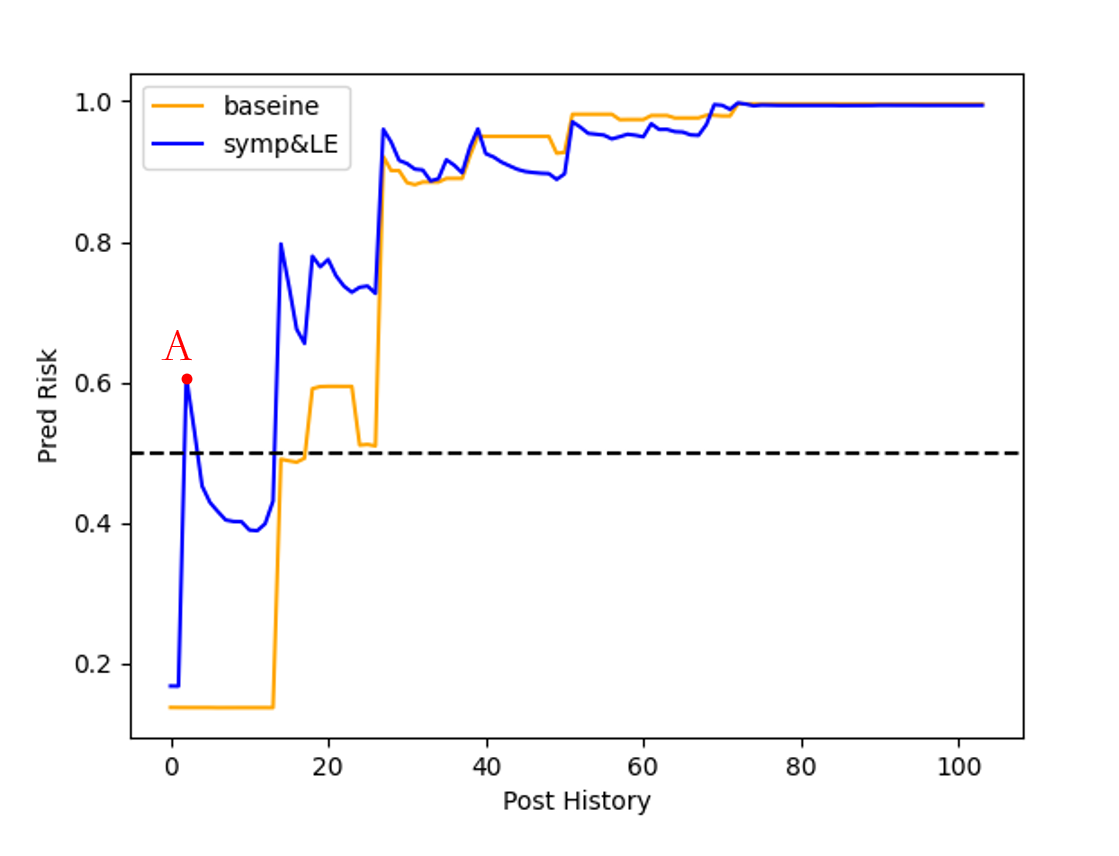
\includegraphics[width=\linewidth]{figures/case_ERD.png}
	\caption{Comparison of the predicted risk along time from two methods on a depression patient in Early Risk Detection. The user has no explicit symptom expression before A, but the symp\&LE method can capture earlier sign from LE.}
	\label{fig:case_ERD}
\end{figure}
\subsection{Diagnosis Point Detection (DPD)}
\paragraph{Dataset} The dataset of this task is RSDD-Time~\cite{macavaney-etal-2018-rsdd}, which has been mentioned in Section \ref{sec:application}. 
The dataset is an annotated corpus sourced from Reddit.  It encompasses two kinds of text spans: diagnoses (e.g., ``I was diagnosed'') and temporal expressions associated with the diagnosis (e.g., ``today''). Consequently, the diagnosis point label can be derived through the utilization of these annotations.

% \MY{Informal expression, rewrite this sentence:} 
% It's an annotated dataset from Reddit, in which two kinds of text spans are annotated: diagnoses (e.g., “I was diagnosed”) and time expressions that are relevant to the diagnosis (e.g., ``today''). Therefore, we can obtain the diagnosis point label using the annotation.   

\paragraph{Baseline} 
% As the DPD task shares lots of similarity with conventional Change Point Detection\MY{if change point detection is never mentioned later, you don't have to abbrev it, super confusing as our task is DPD. You just say the essence is a change point detection problem} 
The essence of our DPD task is the conventional Change Point Detection
Problem~\cite{Truong2020SelectiveRO}, which aims to identify points in a time series indicative of a significant shift in the underlying data distribution. Therefore, we employ \textbf{RuLSIF}~\cite{Liu2013Change}, a well-established CPD model widely recognized for its performance~\cite{hushchyn2021generalization}, as our baseline. RuLSIF\footnote{Relative unconstrained Least Squares Importance Fitting} 
% \MY{This baseline is quite old, 2013, add some arguments say that it still serves well and achieves great performance in a series tasks} 
utilizes a least-squares fitting approach to gauge the dissimilarity between the distributions of successive segments within a time series. When a substantial difference is observed in the distribution between two consecutive segments, a change point is identified. The method offers a non-parametric solution, making minimal assumptions about the underlying data.

\paragraph{Evaluation Metric}
The DPD task aims to identify the exact diagnosis time of an individual, which is quite challenging by analysing the symptom sequences in the posting history. Consequently, applying strict metrics like accuracy and F1 score directly is impractical in this context. To address this, we calculate the F1 score using a smooth time window, defining true positive (TP) samples as those within a specific temporal proximity to the actual diagnosis time. In this study, we set the time window to 30 days, and we refer to this metric as \textbf{$F_1(w=30)$}.

\paragraph{Experiment Results}
Figure \ref{fig:DPD_result} illustrates the experiment results of DPD task. We compare the results of baseline (red line) with causality-enhanced methods in various settings. ``symp'' denotes the inclusion of ``symptom-to-symptom'' causality, ``LE'' indicates the inclusion of ``life-event-to-symptom'' causality, and ``symp\&LE'' encompasses both causality. We can find that causal relationships can significantly improve the detection accuracy of diagnosis point. Interestingly, the ``LE'' causality generally outperforms ``symp'' across all window sizes, and the combination of both causalities shows a substantial improvement, especially with a causal window of 180. 

% We applied the two types of causality using three different interpolation methods to Diagnosis Point Detection. Table \ref{tab:detection_result} shows the results of the baseline model and the results when the results when both types of causality are incorporated. The results are measured using the F1 score. For Table \ref{fig:DPD_result} , the time windows used for the two causality types are consistent (30 days, 90 days, 180 days). From the results, it can be observed that incorporating both types of causality with a time window of 180 days yields the best results, with an F1 score of 38.2.
% \begin{table}[!ht]
%     \small
%     \centering
%     \begin{tabular}{l|c|c}\hline
%     Menthod & Causal Windows & $F_1(w=30)$  \\ \hline
%     RuLSIF & - & 28.8     \\ \hline
%     \multirow{3}*{symp} 
%     & 30  & 30.24  \\
%     & 90  & 31.18  \\
%     & 180  & 30.62  \\
%     \cline{1-3}
%     \multirow{3}*{LE} 
%     & 30 & 33.98 \\
%     & 90 & 32.30 \\
%     & 180 & 32.31 \\
%     \hline
%     \multirow{3}*{symp\&LE}
%     & 30 & 33.71	  \\
%     & 90  & 28.93    \\
%     & 180  & \textbf{38.20}   \\
%     \hline
%     \end{tabular}
%     \caption{}
%     \label{tab:detection_result}
% \end{table}

\begin{figure}[th]
	\centering
	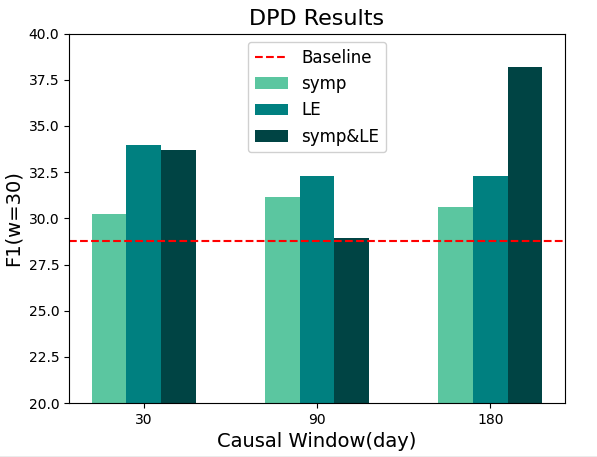
\includegraphics[width=0.9\linewidth]{figures/DPD.png}
	\caption{Results of DPD task. The definition of ``causal window''\textsuperscript{\ref{footnote:causal_window}} can be found in Section \ref{sec:psm}. \textit{symp} is short for ``symptom'', and \textit{LE} is short for ``life event''.}
	\label{fig:DPD_result}
\end{figure}
% \KZ{Missing caption? Also the fonts in some of these figures are too small! Must be at least 3/4 of the size of normal text font.} 





% This suggests the significant role of the introduced causal relationship in enhancing the model's predictive power of future risks.

% Table~\ref{case_ERD_table} presents the posting history of a user before the first peak of the depression risk score. We specifically chose posts mentioning life events.  Users did not immediately mention the symptoms in subsequent posts but rather shared content on other topics, such as game strategies.

% By introducing causal relationships, we successfully detected potential symptoms, enabling us to identify depression risk earlier. This implies that even when users do not explicitly express depressive symptoms, our approach, leveraging the association between life events and symptoms, enables us to sensitively capture latent signs of depression.

% siyuan:baseline只有一个RuLSIF,没有TS-CP2。表格6 7 8应该合并成一张表。
% We applied the obtained causality between symptoms and life events, along with the causality between symptoms, to two downstream tasks. 
% Understanding the causality between symptoms allows us to identify whether the presence of symptom A makes it more likely for symptom B to occur or not. This property can be employed to adjust the probability vector of symptoms (38 dimensions) that changes over time. Let the Causal matrix (38 x 38) be denoted as $C_{symp}$, where $C_{symp}[i][j]$ represents the Average Treatment Effect (ATE) of the i-th symptom causing the j-th symptom. When symptom A appears, according to the Causal matrix, we can determine how much the probabilities of other symptoms increase or decrease. In both of these downstream task, we apply causality through interpolation. $S_D$ refers to the symptom matrix of a user on day D, and $S_D'$ represents the user's symptom matrix after being adjusted by the causal matrix. We adjust the symptom matrix by applying the causal matrix to the average of the matrices from $D-30$ days and $D-1$ day and adding it to the original symptom matrix. The interpolation formula is as follows:
% $$S_D'=S_D+C_{symp}^Tavg(S_{D-30},S_{D-1})$$
% Similarly, we applied the causality between life events and symptoms to the task of time point detection. The interpolation formula is as follows:
% $$S_D'=S_D+C_{LE}^Tavg(L_{D-30},L_{D-1})$$

% Additionally, we incorporate both causal results into two downstream tasks using the method outlined in the formula. $C_{symp}$ and $C_{LE}$ respectively denote the causal matrices between symptoms and between life events and symptoms. Similarly, we adjust the symptom matrix by applying the causal matrix to the average of the matrices from $D-30$ days and $D-1$ day, and the average of life events matrices, and then add it to the original symptom matrix to obtain the adjusted symptom matrix.
% \begin{equation*}
%     \begin{aligned}
% S_D'= S_D+C_{symp}^Tavg(S_{D-30},S_{D-1})
% \\+C_{LE}^Tavg(L_{D-30}, L_{D-1})
% \end{aligned}
% \end{equation*}

% \subsection{Interpolation of causality}
% %baseline:
% Determining the timing of depression is crucial, enabling timely intervention to address the condition or prevent its deterioration. We utilized a classical model for change-point detection, RuLSIF \cite{hushchyn2021generalization}, as baselines. After incorporating causality, we compared the performance in change-point detection. If there is an improvement in the effectiveness of this task, it can also indicate the meaningfulness of the previously obtained causality.
% The baseline for early detection is prior work, psysym\cite{Zhang2022SymptomIF}, an interpretable detection model designed for identifying mental disorders on social media.
